
\vspace{-0.1in}
\section{Causal Framework for Reward Modeling}
\label{sec:preliminaries}

\vspace{-0.05in}
% \begin{figure}[t!]
% \centering
% \includegraphics[width=\linewidth]{images/causalDiagram.pdf} 
% \caption{Conceptual Causal Graph for Reward Modeling. $\mathrm{Q}$ is the query, $\mathcal{I}$ is the latent intent for the response, $\mathcal{U}$ is the set of unknown confounders from the generator, $\mathrm{A}$ is the generated answer, $\mathrm{C}(\mathrm{A})$ are causal attributes, $\mathrm{SP}(\mathrm{A})$ are spurious attributes, and $\mathrm{R}^*$ is the ground-truth reward. The goal is to train $\hat{\mathrm{R}}_\theta$ to estimate $\mathrm{R}^*$, such that its dependence on $\mathrm{A}$ is primarily mediated through $\mathrm{C}(\mathrm{A})$.}
% \label{fig:causal_graph}
% \end{figure}

% \vspace{-0.1in}
% \begin{figure}[t!]
% \centering
% 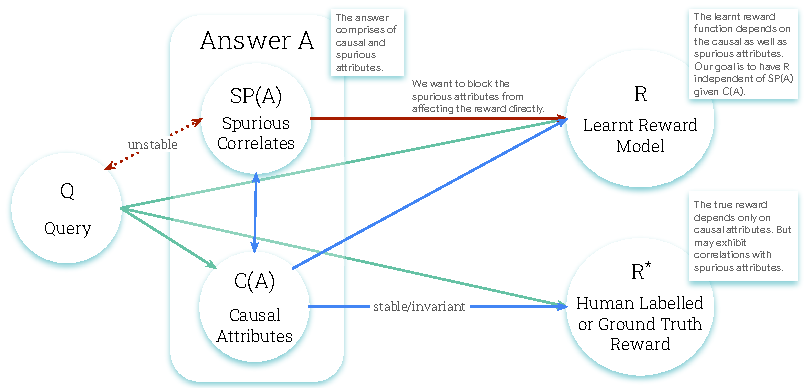
\includegraphics[width=0.7\linewidth]{images/CausalGraphA.pdf} 
% \caption{Conceptual Causal Graph for Reward Modeling. $\mathrm{Q}$ is the query. The Answer (A) comprises of two types of attributes, $\mathrm{C}(\mathrm{A})$, which are causal attributes, and $\mathrm{SP}(\mathrm{A})$ which are spurious attributes. $\mathrm{R}^*$ is the human annotated or ground-truth reward which are posited to depend only on C(A). The goal is to train $\hat{\mathrm{R}}_\theta$ to estimate $\mathrm{R}^*$, such that its dependence on $\mathrm{A}$ is primarily mediated through $\mathrm{C}(\mathrm{A})$. \vspace{-0.2in}}
% \label{fig:causal_graph}
% \end{figure}


\begin{figure}[!t]               % one float, two columns inside
  \centering
  \begin{minipage}[t]{0.58\textwidth}
    \vspace{0.0in}
    \centering
    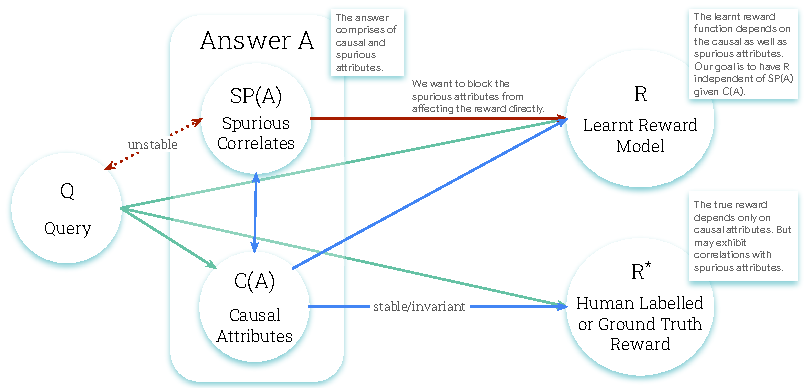
\includegraphics[width=\linewidth]{images/CausalGraphA.pdf}
    % \vspace{-0.1in}
    % \captionof{figure}{Conceptual Causal Graph for Reward Modeling. $\mathrm{Q}$ is the query. Answer (A) has causal attributes $\mathrm{C}(\mathrm{A})$ and spurious attributes $\mathrm{SP}(\mathrm{A})$. Ground-truth reward $\mathrm{R}^*$ depends only on $\mathrm{C(A)}$ and $\mathrm{Q}$. Augmentations heighten $\hat{\mathrm{R}}_\theta$'s sensitivity to $\mathrm{C(A)}$ (approximated by oracle LLM).}
    
  \end{minipage}\hfill
  \begin{minipage}[t]{0.4\textwidth}
        \centering
        \vspace{-0.25in}
        \resizebox{\linewidth}{!}{% Make table fit the minipage width
        \begin{tabular}{c|p{0.75\linewidth}} % Adjusted width for p column, assuming overall table width constraint
\toprule
\textbf{Path/ Relationship} & \textbf{Interpretation Summary} \\
\midrule
$(\mathrm{Q}, \mathrm{C}(\mathrm{A})) \to \mathrm{R}^*$ & Ground-truth reward $\mathrm{R}^*$ determined by query $\mathrm{Q}$ and causal attributes $\mathrm{C(A)}$; stable relationship. \\
$\mathrm{Q} \leftrightarrow \mathrm{SP(A)}$  & Query $\mathrm{Q}$ and unknown spurious attributes $\mathrm{SP(A)}$ are correlated/confounded by unstable exogenous factors. \\
$\mathrm{Q} \to \mathrm{C(A)}$ & Query $\mathrm{Q}$ determines relevant causal attributes $\mathrm{C(A)}$. \\
$\mathrm{SP(A)} \leftrightarrow \mathrm{C(A)}$ & Bidirectional (potentially complex) relationship between spurious $\mathrm{SP(A)}$ and causal $\mathrm{C(A)}$ attributes. \\
\bottomrule
\end{tabular}
        } % End resizebox
        % \vspace{-0.1in}
        % \caption{$\mathrm{R^*} \perp \mathrm{SP(A)} | \mathrm{C(A)}$, Q. $\text{dim}(C(A)) \gg \text{dim}(SP(A)) \forall A$. $\mathrm{SP(A)}$ is unknown. \vspace{-0.2in}}
        \label{tab:causal_arrows}
  \end{minipage}\hfill          % \hfill inserts a flexible gutter
  % \vspace{-0.2in}
\caption{Conceptual Causal Graph for Reward Modeling. $\mathrm{Q}$ is the query. Answer (A) has causal attributes $\mathrm{C}(\mathrm{A})$ and spurious attributes $\mathrm{SP}(\mathrm{A})$. $\text{dim}(C(A)) \ll \text{dim}(SP(A))\ \forall A$. $\mathrm{SP(A)}$ is unknown. Ground-truth reward $\mathrm{R}^*$ depends only on $\mathrm{C(A)}$ and $\mathrm{Q}$ ($\mathrm{R^*} \perp \mathrm{SP(A)} | \mathrm{C(A)}$, Q). Augmentations heighten $\hat{\mathrm{R}}_\theta$'s sensitivity to $\mathrm{C(A)}$ (approximated by oracle LLM).}
\label{fig:causal_graph}
\vspace{-0.15in}
\end{figure}
  % \vspace{0.03in}


% \vspace{-0.1in}
% \begin{figure}[t!]
% \centering
% \includegraphics[width=\linewidth]{images/CausalGraphNew.pdf} 
% \caption{Conceptual Causal Graph for Reward Modeling. $\mathrm{Q}$ is the query, $\mathcal{I}$ is the latent intent for the response, $\mathcal{U}$ is the set of unknown confounders from the generator, $\mathrm{A}$ is the generated answer, $\mathrm{C}(\mathrm{A})$ are causal attributes, $\mathrm{SP}(\mathrm{A})$ are spurious attributes, and $\mathrm{R}^*$ is the ground-truth reward. The goal is to train $\hat{\mathrm{R}}_\theta$ to estimate $\mathrm{R}^*$, such that its dependence on $\mathrm{A}$ is primarily mediated through $\mathrm{C}(\mathrm{A})$.}
% \label{fig:causal_graph}
% \end{figure}

\vspace{-0.05in}
We aim to develop a reward model that accurately assesses the quality of an answer $\mathrm{A}$ provided in response to a query $\mathrm{Q}$. Our approach is grounded in a causal framework designed to distinguish genuine quality drivers from spurious correlates often present in preference data. This involves understanding the answer generation process and strategically augmenting training data with approximated counterfactual examples.

\vspace{-0.1in}
\subsection{Reward Model and Pairwise Preferences}
We train a reward model (RM), denoted $\hat{\mathrm{R}}_\theta(\mathrm{Q}, \mathrm{A})$, to assign a scalar quality score to an answer $\mathrm{A}$ for a query $\mathrm{Q}$. This RM is typically optimized on a dataset  preferences pairs $\mathcal{D}_{\mathrm{pref}} = \{(\mathrm{Q}^{(i)}, \mathrm{y}_w^{(i)}, \mathrm{y}_l^{(i)})\}_{i=1}^N$. Given a pair of answers $(\mathrm{A}_1, \mathrm{A}_2)$, the probability of $\mathrm{A}_1$ being preferred over $\mathrm{A}_2$ is commonly modeled using the Bradley-Terry framework \citep{bradley1952rank}:
\begin{equation}
\mathrm{P}(\mathrm{A}_1 \succ \mathrm{A}_2 | \mathrm{Q}; \theta) = \sigmoid(\hat{s}_\theta(\mathrm{Q}, \mathrm{A}_1) - \hat{s}_\theta(\mathrm{Q}, \mathrm{A}_2)) = \frac{\exp(\hat{s}_\theta(\mathrm{Q}, \mathrm{A}_1))}{\exp(\hat{s}_\theta(\mathrm{Q}, \mathrm{A}_1)) + \exp(\hat{s}_\theta(\mathrm{Q}, \mathrm{A}_2))}
\label{eq:bt_prob_roman}
\end{equation}
where $\hat{s}_\theta(\mathrm{Q}, \mathrm{A})$ represents the underlying scalar score (or logit) assigned by the model to answer $\mathrm{A}$ for query $\mathrm{Q}$. \footnote{The score $\hat{s}_\theta(\mathrm{Q}, \mathrm{A})$ can be the direct output of a reward head or, in some pairwise preference models, $\hat{s}_\theta(\mathrm{Q}, \mathrm{A}_1) - \hat{s}_\theta(\mathrm{Q}, \mathrm{A}_2)$ might be directly modeled as the logit of preferring $\mathrm{A}_1$ over $\mathrm{A}_2$.} The parameters $\theta$ are learned by minimizing the negative log-likelihood of  preferences.

% \subsection{Reward Model and Pairwise Preferences}
% Let $\hat{\mathrm{R}}(\mathrm{Q}, \mathrm{A})$ denote the learned reward model, which assigns a scalar score reflecting the quality of answer $\mathrm{A}$ for query $\mathrm{Q}$. While $\hat{\mathrm{R}}$ provides a pointwise score, it is typically trained using pairwise preference data. Given two answers $\mathrm{A}_1$ and $\mathrm{A}_2$ for the same query $\mathrm{Q}$, we relate the reward scores to preference probabilities using the Bradley-Terry model \citep{bradley1952rank}:
% \begin{equation}
% \mathrm{P}(\mathrm{A}_1 \succ \mathrm{A}_2 | \mathrm{Q}; \theta) = \sigmoid(\hat{\mathrm{R}}_\theta(\mathrm{Q}, \mathrm{A}_1) - \hat{\mathrm{R}}_\theta(\mathrm{Q}, \mathrm{A}_2)) = \frac{\exp(\hat{\mathrm{R}}_\theta(\mathrm{Q}, \mathrm{A}_1))}{\exp(\hat{\mathrm{R}}_\theta(\mathrm{Q}, \mathrm{A}_1)) + \exp(\hat{\mathrm{R}}_\theta(\mathrm{Q}, \mathrm{A}_2))}
% \label{eq:bt_prob_roman}
% \end{equation}
% where $\hat{\mathrm{R}}_\theta$ explicitly denotes the model parameterized by $\theta$, and $\sigmoid(\cdot)$ is the logistic sigmoid function. The parameters $\theta$ are optimized using a dataset of observed preferences $\mathcal{D}_{\mathrm{pref}} = \{(\mathrm{Q}^{(i)}, \mathrm{y}_w^{(i)}, \mathrm{y}_l^{(i)})\}_{i=1}^N$, typically by minimizing the negative log-likelihood based on Eq. \ref{eq:bt_prob_roman}.


% \vspace{-0.15in}
\begin{table}[!t]
\centering
% \caption{Summary of \carma{}'s Synthetic Data Augmentation Strategies using LLM-approximated counterfactuals. $\tilde{\mathrm{A}}^{(C_j \leftarrow target)}$ denotes an LLM rewrite of an original answer $\mathrm{A}$ to set its $j$-th causal attribute $C_j$ to the $target$ state (e.g., "upgraded", "degraded"). 
% $\tilde{\mathrm{A}}_{k}^{(C \leftarrow C(A_m))}$ denotes rewriting answer $A_k$ to match the causal attribute profile $C(A_m)$ of answer $A_m$, while aiming to preserve the spurious attributes $SP(A_k)$ of the original $A_k$.}
\vspace{-0.1in}
\vspace{1em}
\newcolumntype{L}{>{\raggedright\arraybackslash}p{5.0cm}} % Column for "Strategy"
\newcolumntype{P}{>{\raggedright\arraybackslash}p{5.0cm}} % Column for "Generation Pair Example"
\newcolumntype{C}{>{\centering\arraybackslash}p{1.3cm}}  % Column for "Assigned Label"
\newcolumntype{R}{>{\raggedleft\arraybackslash}p{2.5cm}}   % Column for "Training Objective (P_theta)"
\begin{tabular}{@{}l L P C R@{}}
\toprule
\textbf{Category} & \textbf{Strategy} & \textbf{Generation Pair Example} & \textbf{Assigned Label} & \textbf{Training Objective ($\mathrm{P}_\theta$)} \\
\midrule
\multicolumn{5}{l}{\textit{Causal Augmentation} ($\mathcal{D}_{\mathrm{causal}}$) - Enhancing Sensitivity to $\mathrm{C}$} \\
\midrule
Causal & Attribute Upgradation/Degradation & $(\tilde{\mathrm{A}}_{(C_j \leftarrow \text{upgraded})}, \mathrm{A})$ \textbf{or} $(\mathrm{A}, \tilde{\mathrm{A}}_{(C_j \leftarrow \text{degraded})})$ \newline  & $\succ$ & $\to 1$ \\
% Causal & Attribute Degradation & $(\mathrm{A}, \tilde{\mathrm{A}}_{(C_j \leftarrow \text{degraded})})$ \newline \footnotesize{where $\mathrm{A}$ was good on $C_j$} & $\succ$ & $\to 1$ \\
\midrule
\multicolumn{5}{l}{\textit{Neutral Augmentation} ($\mathcal{D}_{\mathrm{neutral}}$) - \textit{Enforcing Invariance to} $\mathrm{SP}$} \\
\midrule
Neutral & Irrelevant Pair Comparison (via Query Change) & $(\mathrm{B}_1, \mathrm{B}_2)$ with irrelevant $\mathrm{Q}_{\text{irrelevant}}$ \newline \footnotesize{s.t. $\mathrm{C(B_1|Q_{\text{irrelevant}})} \approx \mathrm{C(B_2|Q_{\text{irrelevant}})} \approx \mathbf{0}$} & $ \approx $ (tie) & $\approx 0.5$ \\
\bottomrule
\end{tabular}
\caption{Summary of \carma{}'s synthetic data augmentation strategies using LLM-approximated counterfactuals. $\tilde{\mathrm{A}}_{(C_j \leftarrow \text{target})}$ signifies an LLM-generated counterfactual of $\mathrm{A}$ with its $j$-th causal attribute $C_j$ modified.}
\label{tab:augmentation_summary}
\vspace{-0.15in}
\end{table}

\vspace{-0.05in}
\subsection{A Causal Model of Answer Generation}
\label{subsec:causal_graph}

\vspace{-0.05in}
We propose a causal model (Figure \ref{fig:causal_graph}) for answer generation and quality perception. For a query-answer pair $(\mathrm{Q}, \mathrm{A})$, we distinguish two attribute types:

\vspace{-0.1in}
\begin{itemize}[itemsep=0pt,left=0pt]
    \item \textbf{Causal Attributes} $\mathrm{C}(\mathrm{A}) = \{\mathrm{C}_1, \dots, \mathrm{C}_\ell\}$: Fundamental quality dimensions (e.g., factuality, relevance) genuinely determining quality relative to $\mathrm{Q}$.
    \item \textbf{Spurious Attributes} $\mathrm{SP}(\mathrm{A}) = \{\mathrm{SP}_1, \dots, \mathrm{SP}_k\}$: Other features (e.g., length, formatting) correlated with preferences or $\mathrm{Q}$ in $\mathcal{D}_{\mathrm{pref}}$, but not intrinsically determining quality. $\mathrm{SP}(\mathrm{A})$ can be high-dimensional and unknown.
\end{itemize}

\vspace{-0.1in}
The ground-truth reward $\mathrm{R}^*(\mathrm{Q}, \mathrm{A})$ is assumed to be solely a function of causal attributes: $\mathrm{R}^*(\mathrm{Q}, \mathrm{A}) = f^*(\mathrm{Q}, \mathrm{C}(\mathrm{A}))$. This implies conditional independence: $\mathrm{R}^* \perp \mathrm{SP}(\mathrm{A}) | \mathrm{Q}, \mathrm{C}(\mathrm{A})$.

We explicitly assume the following stability property: \textit{If the entire process of answer generation and reward labeling were repeated (e.g., with a different labeler or answer generator), the relationship $(\mathrm{Q}, \mathrm{C}(\mathrm{A})) \to \mathrm{R}^{*}$ determining the reward is stable/invariant.} In contrast, correlations involving $\mathrm{SP}(\mathrm{A})$ (e.g., $\mathrm{SP}(\mathrm{A}) \leftrightarrow \mathrm{C}(\mathrm{A})$ or $\mathrm{SP}(\mathrm{A}) \leftrightarrow \mathrm{Q}$) can arise from various, potentially unstable or unknown exogenous factors, and thus these correlations may vary across such repetitions.

The primary challenge is that standard reward models $\hat{\mathrm{R}}_\theta$ may inadvertently learn high sensitivity to these unstable correlations with $\mathrm{SP}(\mathrm{A})$ (due to its unknown, high-dimensional nature). Our goal is to train $\hat{\mathrm{R}}_\theta$ such that its dependence on $\mathrm{A}$ is primarily mediated through the identified, stable causal attributes $\mathrm{C}(\mathrm{A})$, ensuring robustness to unspecified $\mathrm{SP}(\mathrm{A})$.

% We propose a causal model (Figure \ref{fig:causal_graph}) to analyze the generation of answers and how their quality is perceived. The process begins with a query, answer pair $\mathrm{Q},\mathrm{A}$ that is rated by a human or some other agent providing ground truth reward label. {\color{blue} The answer has two parts, one being causal attributes ($C(A)$) and the other being spurious attributes ($SP(A)$). The reward labeler (or human) uses causal attributes ($C(A)$) to provide ground truth reward label that is part of the training data. All other features are considered to be $SP(A)$ and are correlated with $C(A)$. Further, at the time of answer generation, there may be unknown factors (additional prompts to condition the answer, or unknown exogenous confounding factors) that correlate spurious factors $SP(A)$ with the question. 
% We assume the following: \textit{If the entire process is repeated with different labeler and answer generator, then $Q, C(A) \rightarrow R^{*}$ relationship of reward labeling  is stable/invariant compared to unstable correlation between spurious factors and the question.}}




% \begin{table}[t!]
% \centering
% \caption{Explanation of the Causal Model}
% \label{tab:causal_arrows}
% \vspace{1em}
% \begin{tabular}{c|p{9cm}} % Adjusted widths
% \toprule
% \textbf{Arrow} & \textbf{Interpretation} \\
% \midrule
% $(\mathrm{Q}, \mathrm{C}(\mathrm{A})) \;\to\; \mathrm{R}^*$ & The ground-truth reward $\mathrm{R}^*$ is solely determined by the causal attributes $\mathrm{C(A)}$ and the question $\mathrm{Q}$. The labeling agent is looks  at only $\mathrm{C(A)}$ and $\mathrm{Q}$ to decide on the label. This relationships is assumed to be stable across labeling agents. \\
% $\mathrm{Q}\leftrightarrow \mathrm{SP(A)}$  & $\mathrm{SP(A)}$ - all unknown spurious attributes that is not $\mathrm{C(A)}$ but correlated/confounded with question through unknown factors. This correlation is unstable and is different depending on other exogenous factors.  \\
% $\mathrm{Q}\rightarrow \mathrm{C(A)}$ & Question determines causal attributes of the answer relevant to the reward \\
% $\mathrm{SP(A)} \leftrightarrow \mathrm{C(A)}$ & Causal and spurious attributes have bidirectional relationship. Specifically we will model $SP_1(A) \subseteq SP(A)$ that has no parents in $C(A)$, and $SP_2(A) \subset SP(A)$ with direct parents in $C(A)$ \\

% %$\mathrm{A} \;\to\; \mathrm{C}(\mathrm{A})$ & The answer text manifests causal quality attributes. \\
% %$\mathrm{A} \;\to\; \mathrm{SP}(\mathrm{A})$ & The answer text also manifests spurious attributes. \\
% \midrule
% \multicolumn{2}{p{12cm}}{\textbf{Note:} Key property is the conditional independence $\mathrm{R^*} \perp \mathrm{SP(A)} | \mathrm{C(A)}$. $\mathrm{SP(A)}$ is unknown and potentially very high dimensional ($k >> \ell$). Our augmentation strategies are aimed at heightening sensitivity of reward to $\mathrm{C(A)}$ by varying answers along these only. An approximation to $\mathrm{C(A)}$ is obtained by querying an oracle LLM.  } \\
% \bottomrule
% \end{tabular}
% \end{table} 



\vspace{-0.1in}
\subsection{Approximating Counterfactuals for Attribute Intervention}
\label{subsec:approximating_counterfactuals}
\vspace{-0.05in}

To instill causal sensitivity and spurious invariance in $\hat{\mathrm{R}}_\theta$, \carma{} leverages counterfactual reasoning about how answer quality changes if specific attributes were altered. For an answer $\mathrm{A}$ with attributes $(\mathrm{C}(\mathrm{A}), \mathrm{SP}(\mathrm{A}))$, an ideal counterfactual, $A_{(C_j \leftarrow c'_j)}(u)$, would manifest if only its $j$-th causal attribute $C_j$ were set to $c'_j$, considering its causal effects on other features, while all other exogenous factors $u$ (that produced the factual answer $a$) remained constant. Formally, $P_{U}(A_{(C_j \leftarrow c'_j)}(U) | A(U)=a)$.
% {\color{brown}GP: It would be nice to explain (more clearly) on how the notation should be interpreted. It is not clear at the moment. A few minor issues e.g. the explanation for what ``u'' means comes much later after the variable is introduced.}

As generating such ideal textual counterfactuals is intractable, \carma{} employs Large Language Models (LLMs) to produce \textit{approximations}. These LLM-generated answers, denoted $\tilde{\mathrm{A}}_{(C_j \leftarrow \text{target})}$, are rewrites of an original answer $\mathrm{A}$, prompted to modify $C_j$ (e.g., to a "degraded" state, lowering reward) while aiming for minimal changes to other attributes.



\begin{remark}
For brevity, we denote these LLM approximations as $\tilde{\mathrm{A}}_{(C_j \leftarrow c)}$, dropping the explicit $u$ conditioning, assuming the generation approximates such a sample. While imperfect, these approximations provide the targeted variations crucial for our data augmentation.
\end{remark}

% \vspace{-0.05in}
% \subsection{Construction of Counterfactuals when causal attributes change}
% \label{subsec:approximating_counterfactuals}

% \vspace{-0.05in}
% {\color{blue}
% To train $\hat{\mathrm{R}}_\theta$ for causal sensitivity and spurious invariance, we leverage the concept of counterfactuals: reasoning about how an answer's quality would change if specific attributes were altered. Given an answer $\mathrm{A}$ with attributes $(\mathrm{C}(\mathrm{A}), \mathrm{SP}(\mathrm{A}))$, an ideal counterfactual $A_{(C_j \leftarrow c'_j)} (u)$ would represent $\mathrm{A}$ with only its $j$-th causal attribute $C_j$ changed to $c'_j$ and its effect on other features through their causal relationships, given all else (all hidden factors of variation captured in variable $u$) held in those values that would give rise to the factual answer. Formally, the counterfactual is sampled from $P_{U}(A_{(C_j \leftarrow c'_j)} (U) | A(U) =a)$ - a counterfactual distribution under the exogenous conditional distribution $u$ that gives rise to the factual answer $a$ and under the intervention $(C_j \leftarrow c'_j)$.

% Perfectly constructing such ideal textual counterfactuals is intractable. \carma{} therefore employs Large Language Models (LLMs) to \textit{generate new answers}, denoted $\tilde{\mathrm{A}}_{(\cdot)}$, that \textit{approximate} these ideal counterfactuals. For example, $\tilde{\mathrm{A}}_{(C_j \leftarrow \text{degraded})}(u)$ is an LLM rewrite of the original answer $\mathrm{A}$, prompted to degrade $C_j$, in the sense of lowering the reward, while minimally affecting other attributes. }

% {\color{blue}
% \begin{remark} For the sake of brevity in what follows, we use $\tilde{A}_{C_j \leftarrow c}$ dropping the dependence on exogenous condition $u$ sampled under condition $A(u) = a$. We assume that the generated answer approximately reflects such a sample. While these are approximations and perfect attribute isolation is difficult, they provide the targeted variations necessary for our data augmentation.
% \end{remark}
% }
% \begin{remark}
% In \carma{}, attributes are identified from an existing answer $\mathrm{A}$. An LLM then constructs a \textit{new textual instance} $\tilde{\mathrm{A}}^{(\cdot)}$ to approximate a desired counterfactual state (e.g., $C_j$ modified). 
% \end{remark}

% \subsection{Approximating Counterfactual Answer Variations}
% \label{subsec:approximating_counterfactuals}

% To teach $\hat{\mathrm{R}}_\theta$ the desired sensitivities and invariances, we reason about \textit{counterfactual answers}: what an answer \textit{would have been like} if certain attributes had been different. Given an original answer $\mathrm{A}$ (with its observed attributes $\mathrm{C}(\mathrm{A})$ and $\mathrm{SP}(\mathrm{A})$), we consider an ideal counterfactual, such as $A^{(C_j \leftarrow c'_j)}$, where only the $j$-th causal attribute $C_j$ is hypothetically changed to $c'_j$, while all other causal attributes $\mathrm{C}_{k \neq j}(\mathrm{A})$ and all spurious attributes $\mathrm{SP}(\mathrm{A})$ are held constant.

% Directly constructing such ideal counterfactual answers from a given text $\mathrm{A}$ while perfectly isolating attribute changes is generally intractable. \carma{} employs Large Language Models (LLMs) to \textit{generate new answers} that \textit{approximate} these ideal counterfactuals. We denote these LLM-generated approximations as $\tilde{\mathrm{A}}^{(\cdot)}$. For instance, $\tilde{\mathrm{A}}^{(C_j \leftarrow \text{degraded})}$ is an LLM rewrite of $\mathrm{A}$ that attempts to specifically degrade its quality along the causal attribute $C_j$, with explicit instructions to make "minimal changes" and preserve other attributes as much as possible.

% \begin{remark}
% It is crucial to note that in \carma{}, causal attributes $\mathrm{C}(\mathrm{A})$ and spurious attributes $\mathrm{SP}(\mathrm{A})$ are first identified or inferred \textit{from an existing answer} $\mathrm{A}$. The generation of an approximated counterfactual answer $\tilde{\mathrm{A}}^{(\cdot)}$ is a subsequent step. This new answer $\tilde{\mathrm{A}}^{(\cdot)}$ is constructed by an LLM with the goal of embodying a specific change (e.g., $C_j \leftarrow \text{degraded}$) relative to the original $\mathrm{A}$, while attempting to hold other attributes constant. This process creates a \textit{new textual instance} whose attributes approximate the desired counterfactual state. While perfect isolation is challenging and these are approximations, they provide a valuable training signal for disentangling attribute contributions to the reward.
% \end{remark}

% {\color{blue} KS: Being pedantic, but can someone propagate $\tilde{A}_{C \leftarrow c}$ everywhere. This is just standard convention. So better to simply use the subscript.}

\vspace{-0.1in}
\subsection{Augmented Training Data for Causal Disentanglement}
\label{subsec:data_augmentation}


\vspace{-0.1in}
We augment the original preference dataset $\mathcal{D}_{\mathrm{pref}}$ with synthetically generated examples $\mathcal{D}_{\mathrm{aug}}$ designed to enforce specific causal properties on $\hat{\mathrm{R}}_\theta$. This augmented dataset $\mathcal{D}_{\mathrm{aug}}$ comprises two principal categories: Causal Augmentation Pairs ($\mathcal{D}_{\mathrm{causal}}$) and Neutral Augmentation Pairs ($\mathcal{D}_{\mathrm{neutral}}$), summarized in Table \ref{tab:augmentation_summary}.


\begin{figure}[!t]
  \centering
  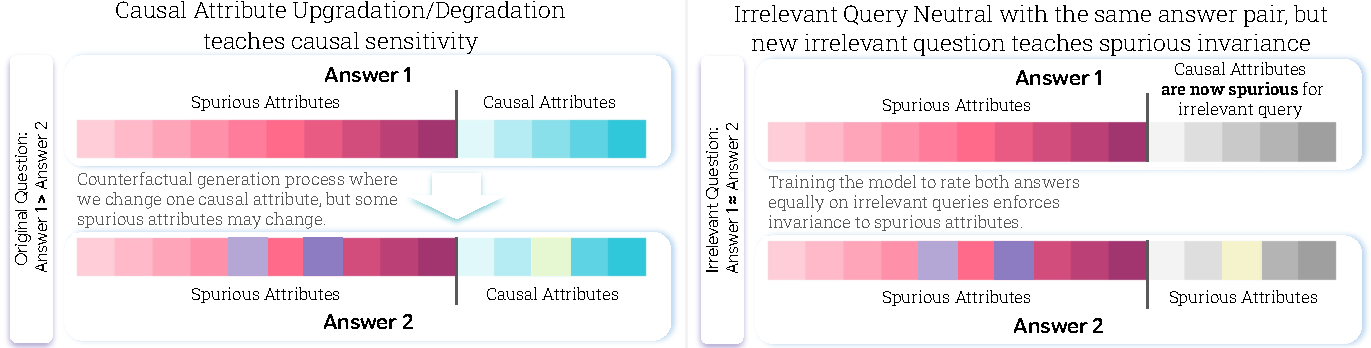
\includegraphics[width=\linewidth]{images/CausalAugmentationProcess_Horizontal.pdf}
  \vspace{-0.2in}
%   \caption{\textbf({Top}) \textit{Causal Augmentation:} LLM-generated counterfactual $\mathrm{A2}$ isolates a change in a causal attribute $\mathrm{C}(\mathrm{A1}|\mathrm{Q})$ of answer $\mathrm{A1}$ for query $\mathrm{Q}$, teaching causal sensitivity.
% ({Bottom}) \textit{Neutral Augmentation:} Answers $\mathrm{A1}$ and $\mathrm{A2}$ are both irrelevant to query $\mathrm{Q}_{new}$, teaching invariance for irrelevant content.}
%   \label{fig:augmentation_strategies_detail}
  \caption{Visualizing \carma's core augmentation strategies (detailed in Appendix~\ref{app:detailed_augmentation_diagrams}).
\textbf{(Top) Causal Augmentation:} For a given query, we use an LLM-driven counterfactual generation process to alter a specific causal attribute, yielding Answer 2. Some spurious attributes may co-vary. The RM is trained with a preference (e.g., $A_1 \succ A_2$ if $A_2$ is a degradation), teaching causal sensitivity.
\textbf{(Bottom) Irrelevant Query Neutral:} The same answer pair ($A_1, A_2$) is re-contextualized with a new, irrelevant question. Their original causal attributes become effectively spurious or irrelevant (greyed-out bar). The RM is trained with a tie-label ($A_1 \approx A_2$), teaching invariance to the  attribute differences when no true causal signal for the current query exists.\vspace{-0.2in}}
\label{fig:carma_augmentation_visual_overview}
  
\end{figure}

% \begin{wrapfigure}{r}{0.6\linewidth}
%     \centering
%     \vspace{-0.5in}
%     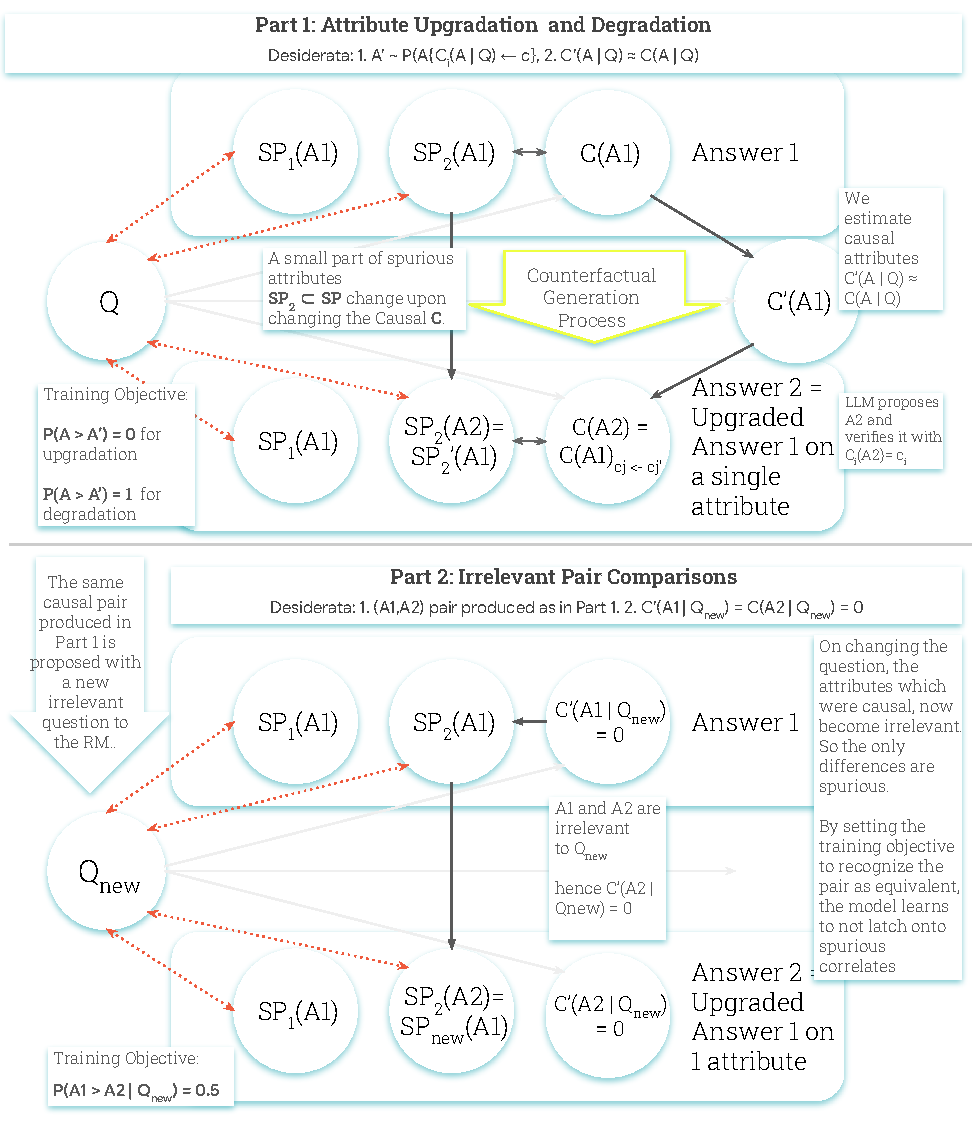
\includegraphics[width=1.0\linewidth]{images/CausalPerturbations.pdf}
%     \vspace{-0.25in}
%     \caption{(\textbf{Top}) \textit{Causal Augmentation:} LLM-generated counterfactual $\mathrm{A}'$ isolates a change in a causal attribute $\mathrm{C}(\mathrm{A}|\mathrm{Q})$ of answer $\mathrm{A}$ for query $\mathrm{Q}$, teaching causal sensitivity.
% (\textbf{Bottom}) \textit{Neutral Augmentation:} Answers $\mathrm{A}$ and $\mathrm{A}'$ (for query $\mathrm{Q}_{new}$) are both irrelevant to query $\mathrm{Q}_2$, teaching invariance for irrelevant content.\vspace{-0.9in}}
%     \label{fig:augmentation_strategies_detail}
% \end{wrapfigure}

% \vspace{-0.05in}



\subsubsection{Causal Augmentation Pairs}
\carma{}'s strategy causal pairs $\mathcal{D}_{\mathrm{causal}}$ focus on isolating the impact of important causal attributes.


% \paragraph{1. Attribute Upgradation.} For an original answer $\mathrm{A}$ (typically a lower-quality response $\mathrm{y}_l^{(i)}$ from $\mathcal{D}_{\mathrm{pref}}$ considered poor on a specific causal attribute $\mathrm{C}_j$), we generate an LLM-approximated counterfactual $\tilde{\mathrm{A}}^{(C_j \leftarrow \text{upgraded})}$ where $C_j$ is improved. The pair $(\tilde{\mathrm{A}}^{(C_j \leftarrow \text{upgraded})}, \mathrm{A})$ is added to $\mathcal{D}_{\mathrm{causal}}$ with the label $\tilde{\mathrm{A}}^{(C_j \leftarrow \text{upgraded})} \succ \mathrm{A}$.


\vspace{-0.1in}
\paragraph{Attribute Upgradation and Degradation.}
For an original answer $\mathrm{A}$ (from $\mathcal{D}_{\mathrm{pref}}$) and a specific causal attribute $\mathrm{C}_j$, we generate LLM-approximated counterfactuals.
If $\mathrm{A}$ is of lower quality regarding $\mathrm{C}_j$, we create an upgraded version $\tilde{\mathrm{A}}_{(\mathrm{C}_j \leftarrow \text{upgraded})}$. The pair $(\tilde{\mathrm{A}}_{(\mathrm{C}_j \leftarrow \text{upgraded})}, \mathrm{A})$ is added to $\mathcal{D}_{\mathrm{causal}}$ with label $\tilde{\mathrm{A}}_{(\mathrm{C}_j \leftarrow \text{upgraded})} \succ \mathrm{A}$ post-verification.
Conversely, if $\mathrm{A}$ is of higher quality on $\mathrm{C}_j$, we generate a degraded version $\tilde{\mathrm{A}}_{(\mathrm{C}_j \leftarrow \text{degraded})}$. The pair $(\mathrm{A}, \tilde{\mathrm{A}}_{(\mathrm{C}_j \leftarrow \text{degraded})})$ is added to $\mathcal{D}_{\mathrm{causal}}$ with label $\mathrm{A} \succ \tilde{\mathrm{A}}_{(\mathrm{C}_j \leftarrow \text{degraded})}$.
These pairs collectively teach $\hat{\mathrm{R}}_\theta$ sensitivity to changes along individual causal dimensions.


% \paragraph{1. Attribute Upgradation.} From a lower-quality answer $\mathrm{A}$ (from $\mathcal{D}_{\mathrm{pref}}$, poor on causal attribute $C_j$), we generate $\tilde{\mathrm{A}}_{(C_j \leftarrow \text{upgraded})}$ where $C_j$ is improved. The pair $(\tilde{\mathrm{A}}_{(C_j \leftarrow \text{upgraded})}, \mathrm{A})$ is added to $\mathcal{D}_{\mathrm{causal}}$ with label $\tilde{\mathrm{A}}_{(C_j \leftarrow \text{upgraded})} \succ \mathrm{A}$, after verification that the causal attribute is indeed improved.




% \vspace{-0.05in}
% \paragraph{2. Attribute Degradation.} Conversely, for an original answer $\mathrm{A}$ (typically a higher-quality response $\mathrm{y}_w^{(i)}$ from $\mathcal{D}_{\mathrm{pref}}$ considered good on $C_j$), we create its approximated degraded version $\tilde{\mathrm{A}}_{(C_j \leftarrow \text{degraded})}$. The pair $(\mathrm{A}, \tilde{\mathrm{A}}_{(C_j \leftarrow \text{degraded})})$ is added to $\mathcal{D}_{\mathrm{causal}}$ with the label $\mathrm{A} \succ \tilde{\mathrm{A}}_{(C_j \leftarrow \text{degraded})}$.
% Collectively, these teach $\hat{\mathrm{R}}_\theta$ to assign higher scores to improvements along specific causal dimensions.

\subsubsection{Neutral Augmentation Pairs}
$\mathcal{D}_{\mathrm{neutral}}$ pairs (with tie-labels) teach invariance to $\mathrm{SP}(\mathrm{A})$ when $\mathrm{C}(\mathrm{A})$ is held constant/ is irrelevant.


% \vspace{-0.1in}
% Given an original preference pair $(\mathrm{A}_1, \mathrm{A}_2)$ from $\mathcal{D}_{\mathrm{pref}}$ (e.g., $\mathrm{A}_1 \succ \mathrm{A}_2$), we prompt an LLM to rewrite $\mathrm{A}_2$ to match the causal attributes of $\mathrm{A}_1$ while attempting to retain the spurious characteristics of $\mathrm{A}_2$, yielding $\tilde{\mathrm{A}}_{2}^{(C \leftarrow C(A_1))}$. The pair $(\mathrm{A}_1, \tilde{\mathrm{A}}_{2}^{(C \leftarrow C(A_1))})$ is labeled as a tie. This strategy is often applied in direct conjunction with original preference data or outputs of causal augmentation, ensuring invariance is learned over relevant attribute distributions.
% \paragraph{1. Causally-Aligned Reconstruction.}
% Given an original preference pair $(\mathrm{A}_1, \mathrm{A}_2)$ (e.g., $\mathrm{A}_1 \succ \mathrm{A}_2$), an LLM rewrites $\mathrm{A}_2$ to match $C(A_1)$ while attempting to retain $SP(A_2)$, yielding $\tilde{\mathrm{A}}_{2(C \leftarrow C(A_1))}$. The pair $(\mathrm{A}_1, \tilde{\mathrm{A}}_{2(C \leftarrow C(A_1))})$ is labeled as a tie. 
% $A_1$ and $\tilde{\mathrm{A}}_{2(C \leftarrow C(A_1))}$ are now (approximately) causally equivalent but differ in their spurious attributes via $SP(A_1)$ vs. $SP(\tilde{\mathrm{A}}_{2(C \leftarrow C(A_1))})$, which is influenced by $SP(A_2)$ as well as confounders $U$ in the new generative process. This effectively enforces invariance learning along these specific spurious variations ($SP(\cdot)$) when causal content is aligned.




% Such an $\tilde{\mathrm{A}}_{2}^{(C \leftarrow C(A_1))}$ is generated through a new model (with different $U$) from the original $A_2$ generator, hence we expect that $SP(A_2) \neq SP(\tilde{\mathrm{A}}_{2}^{(C \leftarrow C(A_1))})$.
% This enforces invariance learning over the spurious features $SP(\cdot)$.

% This enforces invariance learning over the spurious features $SP(\cdot)$.
% This is often applied in conjunction with original or causally manipulated data, ensuring invariance is learned over relevant attribute distributions.


\vspace{-0.1in}
\paragraph{Irrelevant Pair Comparison (via Query Modification).}
We pair two answers, $\mathrm{B}_1, \mathrm{B}_2$ (often from $\mathcal{D}_{\mathrm{causal}}$, e.g., $\mathrm{A}$ and $\tilde{\mathrm{A}}^{(C_j \leftarrow \text{target})}$), with a \textit{new, unrelated query} $\mathrm{Q}_{\text{irrelevant}}$. This makes their causal attributes w.r.t. $\mathrm{Q}_{\text{irrelevant}}$ (i.e., $\mathrm{C(B_1|Q_{\text{irrelevant}})}, \mathrm{C(B_2|Q_{\text{irrelevant}})}$) minimal. The pair $(\mathrm{B}_1, \mathrm{B}_2)$ under $\mathrm{Q}_{\text{irrelevant}}$ receives a tie-label, training the RM to disregard spurious differences when causal relevance is absent. Their causal distinction becomes moot, isolating spurious variations under $\mathrm{Q}_{\text{irrelevant}}$.

% \vspace{-0.1in}
% \paragraph{2. Irrelevant Pair Comparison (via Query Modification).}
% Given two answers $\mathrm{B}_1, \mathrm{B}_2$, we pair them with a new, unrelated query $\mathrm{Q}_{\text{new}}$. Relative to $\mathrm{Q}_{\text{new}}$, both $C(B_1|\mathrm{Q}_{\text{new}})$ and $C(B_2|\mathrm{Q}_{\text{new}})$ become effectively zero (i.e., causally irrelevant). The pair $(\mathrm{B}_1, \mathrm{B}_2)$ for query $\mathrm{Q}_{\text{new}}$ is then labeled as a tie, teaching invariance when causal quality is uniformly low, regardless of variations in spurious features. Concretely, let us say efficiency was a relevant (causal) feature for a coding related question, by swapping out the query, efficiency may become irrelevant. Due to this reason we find (as shown in Section \ref{subsec:experimental_results}) that irrelevant pair comparison is more powerful when done on causal pairs,  since causal pairs differ on only one attribute, which is likely to be irrelevant for a random swapped question. 



\vspace{-0.05in}
Further details on these generation strategies, their relationship with other methods (like Relevance Contrast or direct Spurious Perturbation), and the rationale for \carma{}'s specific choices are discussed in Appendix \ref{sec:causal_model_details}. 
% The combined dataset $\mathcal{D} = \mathcal{D}_{\mathrm{pref}} \cup \mathcal{D}_{\mathrm{causal}} \cup \mathcal{D}_{\mathrm{neutral}}$ (after filtering imperfect augmentations, see Section \ref{subsec:filtering_appendix}) provides the signal for robust training. The central idea is that explicit examples of disentanglement are key to teaching a reward model to distinguish causal quality drivers from spurious correlates. 
We provide the prompts for the generations described in Section \ref{sec:prompt_templates}.